% Define the document class. aastex for manuscript preparation, emulateapj for making it look polished.
% \documentclass[12pt,preprint2]{aastex}
%\documentclass[12pt,a4paper, iop,onecolumn,numberedappendix]{emulateapj}
\documentclass[12pt,preprint]{aastex}

% Import the natbib package for bibliography inclusion. To get it to work right, first typeset the bibliography (BibTex), Command-Shift-B.
% Then, typeset the document with LaTeX, Command-Shift-L or just Command-T.
% To get proper reference citations using aastex (preprint manuscripts), first typeset as emulateapj with BibTex to create the BibTex
% files and then typeset again as aastex to get the manuscript with references.
\usepackage{natbib}
\usepackage{epsfig,graphicx,color}
\usepackage{longtable}
\usepackage{amsmath}

\bibliographystyle{apj}
% A few colors to replace the defaults for certain link types
\definecolor{orange}{cmyk}{0,0.4,0.8,0.2}
\definecolor{darkorange}{rgb}{.71,0.21,0.01}
\definecolor{darkgreen}{rgb}{.12,.54,.11}

%-----------------------------------------------------------------------------
% The hyperref package gives us a pdf with properly built
% internal navigation ('pdf bookmarks' for the table of contents,
% internal cross-reference links, web links for URLs, etc.)
\usepackage{hyperref}
\hypersetup{pdftex,  % needed for pdflatex
  breaklinks=true,  % so long urls are correctly broken across lines
  colorlinks=true,
  urlcolor=blue,
  linkcolor=darkorange,
  citecolor=darkgreen,
  }

%Define this shorthand for scientific notation.
\newcommand{\expnt}[2]{\ensuremath{#1 \times 10^{#2}}}   % scientific notation
\newcommand{\x}{{\bf x}}
\newcommand{\X}{{\bf X}}
\newcommand{\y}{{\bf y}}
\newcommand{\z}{{\bf z}}
\newcommand{\new}{red}
\newcommand{\ptr}{p_{\rm tr}}
\newcommand{\pte}{p_{\rm te}}
\newcommand{\Ex}{\mathbf{E}}
\newcommand{\Prob}{\mathbf{P}}
\newcommand{\PrfL}{\widehat{P}_{\rm{RF,}\mathcal{L}}(y|\x)}
\newcommand{\PrfLx}{\widehat{P}_{\rm{RF,}\mathcal{L}\cup\x'}(y|\x)}
\newcommand{\TreeL}{\theta_{b, \mathcal{L}}(y|\x)}
\newcommand{\TreeLx}{\theta_{b, \mathcal{L}\cup\x'}(y|\x)}
 \def\hipp {{\it Hipparcos~}}


\newcommand{\dd}{\mathrm{d}}

\newcommand{\fobs}{f_i}
\newcommand{\sobs}{s^2_i}

\newcommand{\ftrue}{f_i^*}

% Commands for annotating the docs with fixme and inter-author notes.  See
% below for how to disable these.
%
% Define a \fixme command to mark visually things needing fixing in the draft,
% as well as similar commands for each author to leave initialed special
% comments in the document.
% For final printing or to simply disable these bright warnings, symlink
% (there's a target 'dist_on' in the makefile that does this) the file
% macros_state.tex to macros_off.tex

\newcommand{\fixme}[1] { \textcolor{red} {
{\fbox{ {\bf FIX}
\ensuremath{\blacktriangleright \blacktriangleright \blacktriangleright}}
{\bf #1}
\fbox{\ensuremath{\blacktriangleleft \blacktriangleleft \blacktriangleleft}
} } } }

% And similarly, one (less jarring, with fewer symbols and no boldface) command
% for each one of us to leave comments in the main text.
\newcommand{\james}[1] { \textcolor{blue} {
\ensuremath{\blacklozenge} {\bf james:}  {#1}
\ensuremath{\blacklozenge} } }

\newcommand{\hogg}[1] { \textcolor{darkorange} {
\ensuremath{\blacksquare} {\bf hogg:}  {#1}
\ensuremath{\blacksquare} } }

\newcommand{\dan}[1] { \textcolor{darkgreen} {
\ensuremath{\bigstar} {\bf dan:}  {#1}
\ensuremath{\bigstar} } }

\newcommand{\joey}[1] { \textcolor{red} {
\ensuremath{\clubsuit} {\bf joey:}  {#1}
\ensuremath{\clubsuit} } }%\documentclass[manuscript]{aastex}


\begin{document}
%%%%%%%% TITLE, AUTHORS, PUBLICATION STATUS, and ABSTRACT %%%%%%%%%

\shorttitle{Fitting the Undetected}
\shortauthors{}
\title{Fitting the Undetected:  Light-curve Feature Estimation in the Presence of Non-detections}
\author{
Some wild \& crazy guys
}
%
%\altaffiltext{1}{Astronomy Department, University of California, Berkeley, CA, 94720-7450, USA}
%\altaffiltext{2}{Statistics Department, University of California, Berkeley, CA, 94720-7450, USA}
%\altaffiltext{*}{E-mail: {\tt jwrichar@stat.berkeley.edu}}

% Note the status (in preparation, MNRAS submitted date, ApJ accepted date, in press etc).
\slugcomment{in preparation}


\begin{abstract}
In multi-epoch imaging surveys, faint variable sources will not be
detectable at all epochs.  In principle, the best approach is to
perform photometric measurements anyway, so that there is a datum
recorded at every epoch.  In practice, most surveys only provide
detection upper limits at some epochs; in some not even upper
limits but just the information that the star was not observed.  Here
we demonstrate with real data on periodic variables from the All-Sky
Automated Survey (ASAS) that these non-detections are nonetheless useful in
fitting and parameter estimation; their inclusion improves both
precision and accuracy.  One novel aspect of this work is that we do
not require the data source to include accurate---or even
any---information about the uncertainty variances on detections or the
values of the upper limits; we find that we can model these as latent
variables, even when they are different at every epoch.  Using realistic
simulations of Mira variable stars, we obtain amplitude estimates that
are {\bf XXX\%} more accurate by incorporating the non-detections into
the analysis.  For  Mira and RR Lyrae variables observed by ASAS, our
method obtains a tighter period - amplitude relationship than the standard
technique.
\end{abstract}

%\keywords{stars: variables: general -- methods: data analysis -- methods: statistical -- techniques: photometric}

\section{Introduction}
\label{sec:intro}



Surveys working in real-time tend to analyze each image with an eye to populating databases quickly. Unless a particular region of the sky gets special treatment (such as it is a known place of interest), discovery of variability happens by comparison of flux values at the database level. Analysis on such databases of transient/variables thus deals with censored data where there is often less information available than there should be. Even then, we might be able to infer what the thresholds were based on S/N measurements of objects neighboring the source of interest.


\joey{What people actually do, what problems that could cause, and what people should do}

A photometric survey (think of it as operating in a single photometric
bandpass for now) scans over the celestial position of a particular
variable star  a large number of times $t_i$.  At each of these
times, the imaging data are analyzed by software, which
treats each scan as a \emph{completely independent} survey.  That is,
when analyzing the data from time $t_i$, none of the information from
any of the other times is used in any way.




At each time $t_i$, the star is either detected by the
software or not.  When it is detected, the software returns
a (possibly bad) flux value $f_i$ and (likely bad) uncertainty
variance $s_i^2$.  When the source is \emph{not} detected,
nothing is reported---in this case, because the software is not
awesome, it doesn't see any reason to report anything at all, since on
the non-detect passes, it has no inkling that this patch of the sky is
interesting in any way.  Welcome to the desert of the real.

Beyond this, there are two additional issues.  The first is that each
night of imaging is different in an unreported and unknown way.  That
is, there is different transparency, sky brightness, and point-spread
function.  So the detection limit, or completeness level, or censoring
of the catalog is different every night.  The second issue is that
either because we are getting the data from a non-generous source, or
because the conditions change rapidly and unpredictably, we can't
analyze all the sources in a finite patch simultaneously.  For each
variable star of interest, we \emph{only} get the data on that star
itself.

\joey{RRL end at 120 kpc in Sesar et al. paper}

\joey{discuss in context of: parameter estimation (amplitude / period), discovery (we're gonna find a lot more variable sources if we take the non-detections into account), and classification; lossiness}

\joey{let's make a point to stress variable discovery}

\joey{Numbers of LCs affected: Stripe 82, ASAS}




\section{Formulating the Model}
\label{sec:model}

%This note, based on the original note from JWR on Feb. 8, 2012, includes revisions from David Hogg, James Long, Nat Butler, and Josh Bloom.

As a reminder, we are modeling light curve data in the presence of non-detections, which are epochs of observation in which no detection of the source of interest was made.

\subsection{Preliminaries}
\label{ss:prelim}

For each astronomical object, a photometric survey measures a multi-epoch light curve over $N$ (typically unevenly spaced) epochs.  At each epoch $i$, with associated time $t_i$, the survey takes an exposure at the location of the object and either (a) detects the object and records an estimate of its photon flux, $\fobs$ and the  variance of the statistical uncertainty in that estimate, $\sobs$, or (b) fails to detect the object.  In the latter case, most modern surveys either record a reference value to signify that no detection was made (as is done in ASAS) or an estimate of the upper detection limit, $b_i$, which is the minimum brightness that could have been detected.

There are many reasons that a source might not show up in a catalog.  These include:
\begin{itemize}
\item low S/N of the source, due either to a higher noise level or a fainter signal,
\item the source falling outside of the detection window (e.g., near chip edge),
\item occulting of the source by an artifact of the detector (e.g., hot pixels, masked out), or
\item the source was out-shone by an intervening object (e.g., asteroid, comet, variable star, airplane, etc.).
\end{itemize}
Here, we present a statistical model that can be used to detect variable sources and model their variability using multi-epoch light curves containing epochs of non-detection.  Previous efforts to detect and model variability using multi-epoch photometry have typically ignored non-detections (REFs) or used them in an ad-hoc manner lacking statistical rigor (REFs).  An exception is \citet{2009AJ....137.4400L}, who measure proper motions of sources in SDSS falling below the detection limit.


In this paper, we will assume that $\fobs$ and $\sobs$ take on real-valued numbers in epochs for which the source was detected and receive the reference value {\tt NA} in epochs where no detection was made. For notational convenience we assemble all the light curve data for one source into a data set $D$ given by
\begin{eqnarray}\displaystyle
D &\equiv& \{D_i\}_{i=1}^N
\\
D_i &\equiv& (\fobs, \sobs)
\quad ,
\end{eqnarray}
where $(\fobs, \sobs)$ are the light curve measurements  at $t_i$.  The goal, for each astronomical object, is to construct the likelihood for the data $D$, given a set of model parameters that describe the variability of the object and the characteristics of the observations, and then to maximize the likelihood with respect to the model parameters.% or to use it in further inference.


\section{The Light Curve Model}
\label{sec:model}
\subsection{Modeling Non-Detections}
To model the mean brightness of the light curve as a function of time, we use a multiple-harmonic Fourier model with angular oscillation frequency $\omega$,
\begin{eqnarray}\displaystyle
\mu_i' &=& A_0 + \sum_{k=1}^K A_k\, \sin (t_i \, \omega  k) + B_k\, \cos (t_i \, \omega  k)
\quad ,\label{eq:fourier}
\end{eqnarray}
where $\mu_i'$ is the model brightness estimate in magnitude at time $t_i$, $\sqrt{A_k^2 + B_k^2}$ is the amplitude of the $k^{\rm th}$ harmonic of the frequency $\omega$ and $\tan^{-1}(\frac{B_k}{A_k})$ is the relative phase offset of harmonic $k$.  The number of harmonics, $K$, can either be fixed or treated as a free parameter over which to optimize the likelihood.

We model the brightness in magnitude because periodic variation in magnitude is more sinusoidal than in flux. However since errors are more Gaussian in flux space, we convert the $u_i'$ to flux measurements using
\begin{equation*}
\mu_i = 10^6 \times 10^{-.4 \mu_i'}
\end{equation*}
Now both the model predictions $\mu_i$ and the data $(f_i,s_i)$ are in flux.

In addition to the expected brightness in Equation \ref{eq:fourier}, we assume that there is uncertainty or inappropriateness in the model, leading to a \emph{fractional model variance} $\eta^2$ at each point (assumed constant but easily generalized) as well as random variation due to photon arrival counts, assumed normal mean 0 with variance $\sigma_i^2$. The reported uncertainties $s_i^2$ are an estimate of the $\sigma_i^2$, see Subsection \ref{sec:uncertainty}. This leads to a true flux measurement of
\begin{eqnarray}\displaystyle
\ftrue = \mu_i + e_i
\label{eq:truefluxdef}
\end{eqnarray}
where $e_i \sim N(0,\sigma_i^2 + \eta^2\,\mu_i^2)$. Recall that $f_i^*$ is a latent variable because we will not see it when an observation is censored. We instantiate a latent variable, $b_i$, to represent the detection limit, in units of flux, at epoch $i$.  The $b_i$ parameter is essential because it probabilistically constrains the possible values of the mean brightness, $\mu_i$, of the light curve when there is a non-detection.  By employing a hierarchical model for the distribution of $b_i$, we can fully utilize all of the information encoded in both the detections and non-detections when computing the data likelihood.   At each epoch, we connect the observed flux, $\fobs$, to the latent variable $\ftrue$ by
\begin{eqnarray}\displaystyle
\fobs &=& \left\{\begin{array}{ll}
  \ftrue & \mbox{if $\ftrue \ge b_i$} \\
  \texttt{NA} & \mbox{if $\ftrue < b_i$} \\
\end{array} \right.
\end{eqnarray}
The observed flux is \texttt{NA} only when the true flux, $\ftrue$, is below the detection limit $b_i$.

Using the model above, the likelihood of the observed $\fobs$ given $\sigma^2_i$, $\theta$ and $I$ (after integrating out the unknown $b_i$) is
\begin{eqnarray}\displaystyle
p(\fobs |\sigma^2_i,\theta,I) &=& \left\{\begin{array}{ll}
  N(\fobs | \mu_i,  \sigma^2_i + \eta^2\,\mu_i^2)\,  \int_{-\infty}^{\fobs} p(b_i | \theta)\, \dd b_i & \mbox{if $\fobs \ne \texttt{NA}$} \\
  \int_{-\infty}^{\infty} \int_{-\infty}^{b_i} N(\ftrue | \mu_i, \sigma^2_i + \eta^2\,\mu_i^2)\, p(b_i | \theta)\, \dd \ftrue\, \dd b_i & \mbox{if $\fobs = \texttt{NA}$} \\
\end{array}\right.\label{eq:mlik}
\\
p(b_i|\theta) &=& N(b_i|B,V_B)
\label{eq:bprior}
\\
\theta &\equiv& (\omega, A_0, \{A_k, B_k\}_{k=1}^K, \eta^2, B, V_B, \cdots) \quad ,
\end{eqnarray}
where we have introduced the hyperparameters $B$ and $V_B$ for the Gaussian prior distribution of $b_i$.  In Equation \ref{eq:mlik}, in the epochs for which a detection was made ($\fobs \ne \texttt{NA}$), we marginalize over the unknown $b_i$ up to the observed flux $\fobs$, enforcing that the detection limit be fainter than the observed brightness. Computationally, this requires a call to a Gaussian pdf, a call to a Gaussian cdf, and a multiplication. In the epochs for which no detection was made ($\fobs = \texttt{NA}$), we compute the probability that the unknown detection threshold $b_i$ is greater than the unknown true flux $f_i^*$. When both $b_i$ and $f_i^*$ are normally distributed, this can be computed using a single call to a Gaussian cumulative distribution function.

In the above, we have assumed no extra information on each of the $b_i$ values besides the knowledge of whether a detection was made at that epoch.  Hence, we draw, in Equation \ref{eq:bprior}, each $b_i$ value from a global prior distribution which is the same at all epochs.  If instead, we are given an estimate of $b_i$ plus its error distribution for each epoch (which, in principle can be inferred from the raw telescope images), we can replace Equation \ref{eq:bprior} with a different distribution per epoch.  In the case that the $b_i$ are assumed to be completely known (without error), the data likelihood of $\fobs$ becomes
\begin{eqnarray}\displaystyle
p(\fobs |\sigma^2_i,\theta,I, b_i) &=& \left\{\begin{array}{ll}
  N(\fobs | \mu_i,  \sigma^2_i + \eta^2\,\mu_i^2)\,  I(\fobs \ge b_i) & \mbox{if $\fobs \ne \texttt{NA}$} \\
 \int_{-\infty}^{b_i} N(\ftrue | \mu_i, \sigma^2_i + \eta^2\,\mu_i^2)\, \dd \ftrue & \mbox{if $\fobs = \texttt{NA}$} \\
\end{array}\right.\label{eq:mlik_s}
\quad ,
\end{eqnarray}
where the boolean indictor function, $I(\ftrue \ge b_i)$, is 1 if $\ftrue \ge b_i$ and 0 otherwise.



\subsection{Modeling Uncertainty in Uncertainties}
\label{sec:uncertainty}
Instead of assuming that $\sobs$ is a perfect, error-free measurement, we probabilistically connect it to the true photon count uncertainty variance $\sigma^2_i$ through a Gamma likelihood.  Our probability of observed $\sobs$ given $\fobs$, $\sigma^2_i$, $\theta$ and $I$, is
\begin{eqnarray}\displaystyle
p(\sobs | \fobs, \sigma^2_i, \theta,I) &=& \left\{\begin{array}{ll}
  \Gamma (\sobs | \sigma^2_i, V_{\sigma} ) & \mbox{if $\fobs \ne \texttt{NA}$} \\
 I(\sobs = \texttt{NA})& \mbox{if $\fobs = \texttt{NA}$}
\end{array}\right.\label{eq:slik}
\quad ,
\end{eqnarray}
where $\Gamma(x | m, V)$ is the standard Gamma distribution parameterized by its mean $m$ and variance $V$.
The  model parameter $V_\sigma$ represents the
variance in the distribution of reported uncertainties given the true
uncertainty.  (Typically, the Gamma distribution is parameterized by parameters $(\alpha, \beta)$, where the mean is $\alpha\beta$ and the variance is $\alpha\beta^2$.)  The  purpose of
 including the likelihood in Equation \ref{eq:slik} to the model, in practice, is to keep the $\sigma^2_i$ from
drifting very far away from the $\sobs$, as set by the hyperparameter
$V_\sigma$. \james{maybe clarify this last sentence. isn't the main reason for having the $V_\sigma$ term because we don't believe the reported variance}

We place a Gamma prior on the true photon count uncertainties, adding two parameters to our model.
\begin{eqnarray}\displaystyle
p(\sigma^2_i|\theta, I) &=& \Gamma(\sigma^2_i | S, V_S)
\label{eq:sigma_prior}
\end{eqnarray}
\james{should probably justify choice of some priors here / include some plots and/or refs. gamma priors and normal priors.}

\subsection{The Full Model}
\label{sec:full}
Putting it all together, we can write down the likelihood of the data, $D_i$, for the parameters $\theta$, on a single epoch, as
\begin{eqnarray}\displaystyle
p(D_i|\theta,I) &=& \int_0^{\infty} p(\fobs |\sigma^2_i,\theta,I)\, p(\sobs | \fobs, \sigma^2_i,\theta,I)\, p(\sigma^2_i | \theta, I)\,\dd \sigma^2_i
\\
\theta &\equiv& (\omega, A_0, \{A_k, B_k\}_{k=1}^K, \eta^2\,\mu_i^2, B, V_B, V_{\sigma}, S, V_S) \quad ,
\end{eqnarray}
where we have inserted the expressions from Equations (\ref{eq:mlik}), (\ref{eq:slik}), and (\ref{eq:sigma_prior}), and integrated over the nuisance parameter $\sigma^2_i$.

Finally if we assume that the data collected at each epoch are independent given the model parameters, we have that
\begin{eqnarray}\displaystyle
p(D|\theta,I) &=& \prod_i p(D_i|\theta,I)
\quad.
\end{eqnarray}
This is the likelihood for the entire
data set (all the measurements and non-detections of this star from
all the epochs, as delivered by the survey) given the $2K + 9$ parameter vector $\theta$.
Figure \ref{fig:graph} displays a graphical model highlighting dependencies and 
independence assumptions. This model
``correctly'' or at least ``justifiably'' uses all of the information
available, without making strong assumptions about the survey or its
veracity.

\begin{figure}[hbtp]
  \begin{center}
    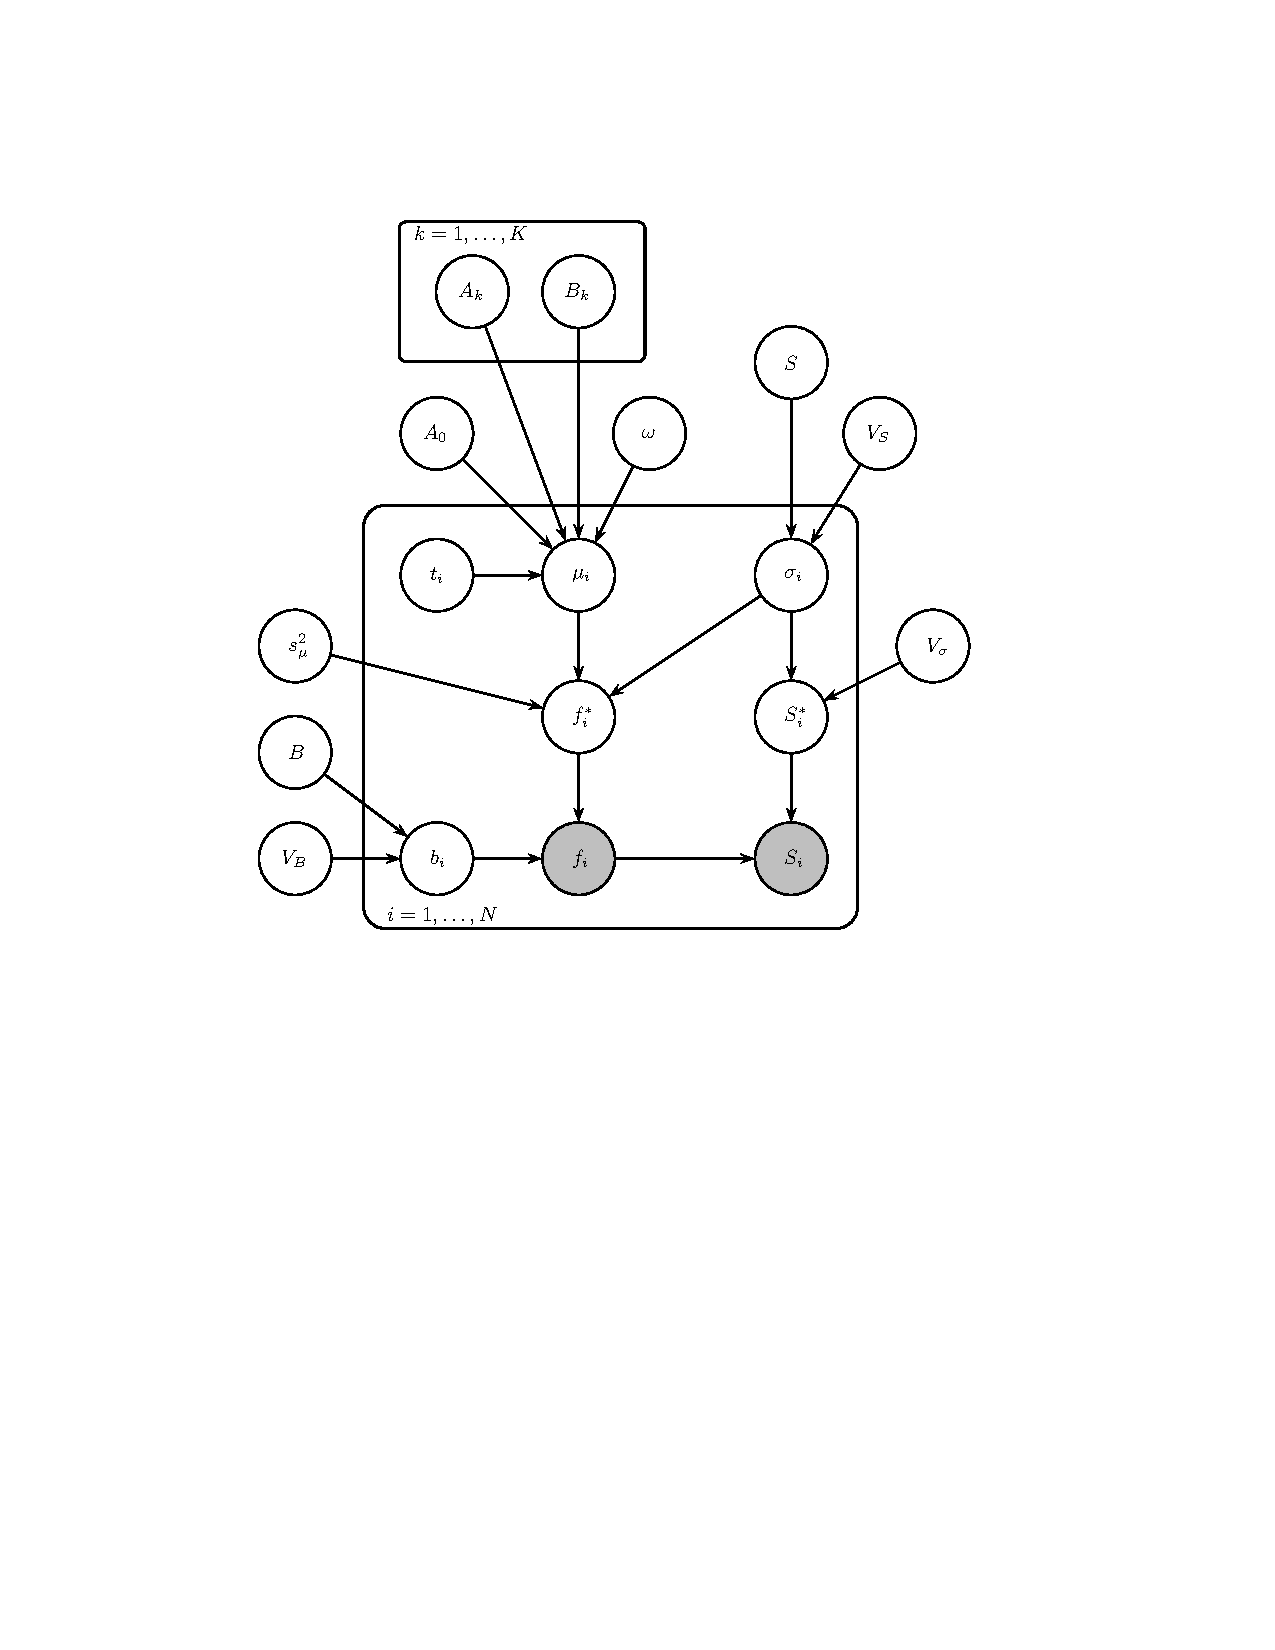
\includegraphics[width=\textwidth,%
      trim=3cm 12cm 5cm 3cm, clip=true]{gm/gm.pdf}
  \end{center}
  \caption{The graphical representation of the probability distribution.
    \label{fig:graph}}
\end{figure}

\subsection{Optimization in Practice}
\label{ss:optim}



\joey{Describe how we optimize}




\section{Experiments}
\label{sec:experiments}

\joey{Note: ASAS provides periods and amplitude for all of the objects in ACVS!  We can and should use this as a comparison set}

\joey{From a brief reading of a few Mira papers, it seems that some papers throw away Miras for which no trough of the LC was observed.  This seems silly.  I have an idea of the P-A plots from Hipparcos.  Should be a good comparison set.  Also, we can consider applying this to Hipparcos, which has publicly available data.}

\subsection{Simulating Faint Mira Variables}
\label{ss:mirasim}

In this first experiment, we begin with a well-observed Mira variable from the ASAS Catalog of Variable Stars (ACVS, \citealt{acvs}) , ASAS 235627-4947.2.  This star has a pulsation period of 266.6286 days and a Lomb-Scargle amplitude of 2.38 mag (V band).  Note there are no non-detections in the ASAS light curve.

To simulate faint Mira stars from ASAS 235627-4947.2, we use the following procedure:
\begin{enumerate}
\item Convert the observed magnitudes $m_i$ and uncertainty variances $s^2_{m,i}$ to fluxes $f_i$ and flux uncertainty variances $s^2_{f,i}$ (we assume a V-band zero-point of $3.67\times10^{-9}$ erg/s/cm$^2$/\AA)
\item For a given flux dimming parameter, $d$, sample the new fluxes, $\tilde{f}_i$, from a Gaussian distribution centered around $f_i / d$ with standard deviation sampled from the empirical ASAS distribution of $s^2_{f,i} | f_i$. \joey{I found that relationship to be linear with a slope $\approx 1$, which is probably BS since the ASAS mag errors are all crap.  So I added a reference value to each flux error to ensure a mag limit $\approx$ 14.5 mag.}
\item Fluxes that are not at least 5$\sigma$ above zero are denoted as non-detections and their flux estimates (and errors) are censored.
\end{enumerate}
Folded light curves of ASAS 235627-4947.2, dimmed by four different values of $d$, are plotted in Figure \ref{fig:mirasim}.


\begin{figure*}
\begin{center}
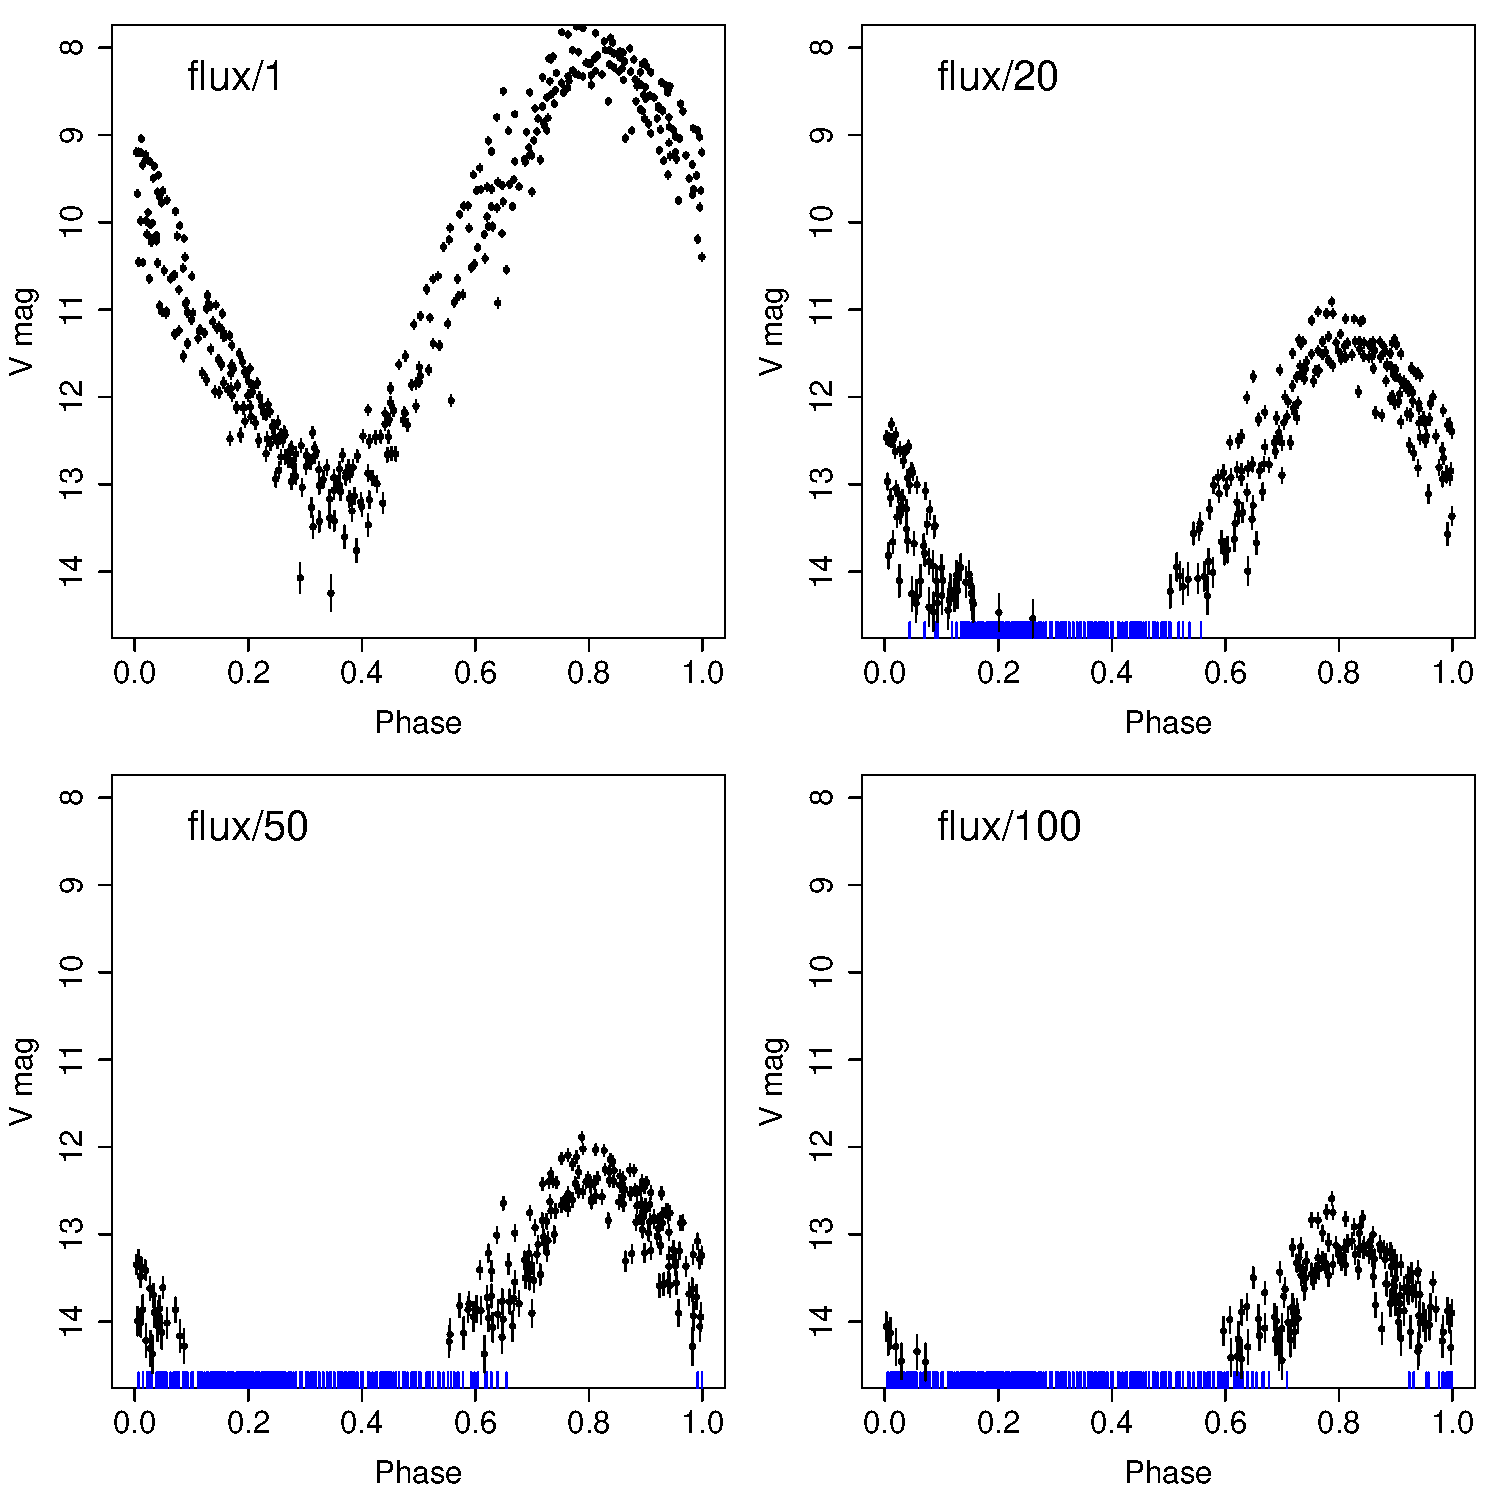
\includegraphics[angle=0,width=6.5in]{../plots/mira_simulated.pdf}
\end{center}
\caption{ Folded light curves for data simulated from the Mira variable ASAS 235627-4947.2 using the prescription in \S\ref{ss:mirasim}.  Blue tick marks along the bottom axis denote phases where there were non-detections.  As the original flux measurements are dimmed by higher factors, the troughs of the sinusoidal light curve are censored, resulting in an incomplete view of the data.  \label{fig:mirasim}}
\end{figure*}


\subsection{Results of Fitting Miras}


\section{Results: ASAS Light Curves}
\label{sec:results}

We use the methodology of \cite{2011arXiv1106.2832R} to select the top ASAS Mira  and RR Lyrae, Fundamental Mode candidates.  Using a posterior probability threshold of 0.8 gives us 1720 Mira  and 1029 RR Lyrae candidates.

 \subsection{Mira Variables}

 Show P - A relationship before and after using the method



 \subsection{RR Lyrae Variables}

  Show P - A relationship before and after using the method

There is an RRL P - A relationship (strong linear anti-correlation)


\section{Discussion}
\label{sec:discussion}

What people can do, starting from the data-taking procedure.

limitations



\acknowledgements


\bibliography{non_detect}

\end{document}
